\chapter{Works Done}
\section{What we did}
Durant les deux mois et demi de ce projet, nous avons implémenté les deux modèles qui étaient décrit dans l'article. Pour rappel, ces deux modèles sont un random simple et un modèle concernant des phéromones. Dans cette rubrique, nous allons vous expliquer le travail de développement que nous avons fourni et les différents choix effectués. Nous n'avons pas trouvé d'utilité à faire un diagramme UML vu la simplicité de l'architecture.\\\\

During two and a half months of this project, we implemented both models which were described in the article. As a reminder, these two models are a simple random and a model concerning pheromones.We also implemented the Random Waypoint model on the demand of our customers. In this section, we are going to explain you the work of development which we supplied and the various made choices. We did not find utility to make a UML diagram seen the simplicity of the architecture.\\\\

\subsection{random model} 

Pour implémenter ce modèle, nous avons eu besoin de trois classes.\\
La première classe, qui se nomme Main.java, permet comme son nom l'indique de lancer le programme. C'est dans cette classe que nous définissons la taille de la fenêtre, la matrice qui servira à simuler le scan d'une zone (tous les noeuds auront la même matrice), et l'instanciation des différents objets provenant de la librairies JBotSim. Nous avons par exemple, un objet s'intitulant \textit{topo} qui est une topology. Cet objet est la base pour notre simulateur. C'est à cette topology que l'on va pouvoir ajouter des nœuds mobiles (ici des avions).\\

To implement this model, we needed three classes. \\
The first class, which is called \textit{Main.java}, allows as its name indicates it launching the program. It is in this class that we define the size of the window, the matrix which will serve to feign the scan of a zone (all the nodes will have the same matrix), and the instanciation of the various objects coming of JBotSim library. We have for example, an object being entitled \textit{topo} which is a topology. This object is the base(basis) for our simulator. It is to this topology that we are going to be able to add mobile nodes (here planes). \\

Nous avons aussi instancié un objet de type Jtopology. Nous expliquerons ce choix dans la suite de la présentation des classes.\\\\
La deuxième classe de notre architecture se nomme \textit{MovingNode}. C'est dans cette classe que sera traité le mouvement des différents nœuds. Cette classe hérite donc de la classe \textit{Node} et implémente l'interface \textit{ClockListesner}, toutes les deux provenant de la librairie JBotSim. Elle hérite de la classe \textit{Node} car les avions seront représentés par des nœuds mobiles, il nous faut donc les caractéristiques de ceux-ci. De plus, elle implémente l'interface \textit{ClockListener} car nous avons besoin que nos nœuds bougent tout les certains temps, on a donc besoin d'un clock d'horloge pour réaliser cela. Nous aurons donc un listener pour le temps, ainsi qu'une méthode \textit{onClock} qui sera appelée à chaque top d'horloge.\\\\

We also instantiated an object Jtopology's object type. We shall explain this choice during the presentation of classes. \\\\
The second class of our architecture is called \textit{MovingNode}. It is in this class that will be handled the movement of the various nodes. This class thus inherits from the class \textit{Node} and implement the interface \textit{ClockListesner}, both resulting(coming) from the JBotSim. It inherits from the class \textit{Node} because planes will be represented by mobile node, we thus need the characteristics of these. Furthermore, It implements the interface \textit{ClockListener} because we need that our nodes move all the seconds, we thus need a top of clock to realize it. We shall thus have a listener for time , as well as a method \textit{onClock} which will be called to every top of horloge. \\\\


Cette classe contient un constructeur par défaut, permettant d'instancier et d'initialiser les différents variables, et d'associer des images aux noeuds mobiles (appel de la méthode \textit{setProperty}. Le modèle random a pour caractéristique de n'avoir aucune communication entre les différents noeuds. Pour réaliser cela, nous passons un argument valant \-1 à la méthode \textit{setCommunicationRange}.\\\\
Comme indiqué dans l'article, les noeuds du modèle random changent d'actions toute les secondes en fonctions de la dernière action entreprise. Pour rappel, voici la table d'action pour le modèle random : \\\\

This class contains a constructor by default, allowing to instantiate and to initialize the various variable, and to associate images with the mobile nodes (call of the method \textit{setProperty}. The random model has for characteristic to have no communication between the various nodes. To realize it, we cross a being worth argument \-1 in the method \textit{setCommunicationRange}. \\\\
As indicated in the article, the nodes of the random model change actions quite the seconds in functions of the last undertaken action. As a reminder, here is the table of action for the random model: \\\\
\begin{center}
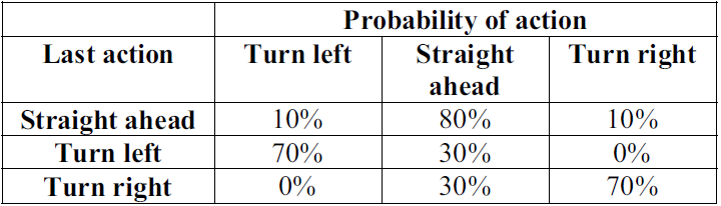
\includegraphics{../images/table_random.png}
\end{center}

Dans notre implémentation, nous avons donc une variable \textit{lastdirection} permettant de savoir la dernière action qui a été faite. Nous avons associé des chiffres aux dernières actions de faite. Si la dernière direction était la gauche, alors la variable \textit{lastdirection} prend la valeur 1, si elle était tout droit, alors on lui associe la valeur 2, et si c'était à droite, on lui associe la valeur 3.\\\\

In our implementation, we have a variable \textit{lastdirection} allowing to know the last action which was made. We associated figures with the last actions of made. If the last direction was the left, then the variable \textit {lastdirection} takes the value 1, if it was quite right, then we associate the value 2, and if it was to the right, we associate the value 3. \\\\

Pour respecter le plus possible la réalité, nous avons dû modifier la gestion des bords de la fenêtre. En effet, à l'origine dans JBotSim, les noeuds peuvent passer d'un bord à l'autre. Par exemple, s'ils atteignaient le bord gauche, ils se retrouvaient par la suite à droite de la fenêtre, ce qui n'est pas possible dans la vie réelle. Nous avons donc bloqué ce problème en rectifiant les coordonnées du noeud, et en changeant son angle de direction. \\\\

To respect as much as possible the reality, we had to modify the management of the edges of the window. Indeed, originally in JBotSim, nodes can pass from an edge to the other one. For example, if they reached the left edge, they found themselves afterward to the right of the window, what is not possible in the real life. We blocked this problem by rectifying the position of the node, and by changing its angle of direction. \\\\

A chaque fois qu'un noeud scanne une zone, il regarde dans la matrice si cette position a déjà été scanné (0 si la zone n'a jamais été scanné, 1 sinon). Si c'est le cas, alors il ne fait rien, sinon il met la valeur à 1.\\\\

La troisième classe de notre architecture se nomme \textit{Jtopology\_Random}. Elle hérite de JTopology et va permettre de dessiner les traces des scans sur la map. Cette classe JTopology hérite de JPanel, et se situe en fait entre une JViewer et une Topology.\\\\

Every time a node scans a zone, it looks in the matrix if this position was already scanned (0 if the zone was never scanned, 1 otherwise). If it is the case, then it makes nothing, otherwise it puts the value to 1. \\\\

The third class of our architecture is called \textit{Jtopology\_Random}. It inherits from JTopology and is going to allow to draw the tracks of scans on the map. This class JTopology inherits from JPanel, and is situated in fact between a JViewer and a Topology.

\subsection{Random Waypoint Model}

This model is very similar to the previous. The only difference is their way to move. \\In this model, the node choose one point randomly and move to it. \\So the only modification compared to the previous model is the class \textit{MovingNode} and more precisely the method \textit{on clock}.


\subsection{Pheromone model}
Au niveau architecture, l'implémentation du modèle des phéromones est très similaire. On retrouve pratiquement les 3 même classe. Seulement la classe \textit{MovingNode} va réellement être différente car les mouvements des noeuds vont dépendre de beaucoup de paramètre. Tout d'abord, cette classe implémente une interface de plus qui est \textit{MessageListener}. En effet, dans ce modèle, les noeuds vont devoir se transmettre des données (en l'occurrence leur map respective).\\\\

La méthode qui va changer le plus par rapport au modèle aléatoire est la méthode \textit{onClock}. En effet, c'est ici que l'on va appliquer les règles comme décrites sur l'image suivante : \\\\

Concerning the architecture, the implementation of the model of pheromones is very similar. We find practically 3 even classy. Only the class \textit{MovingNode} is really going to be different because the movements of nodes are going to depend on a lot of parameter. First of all, this class implements an interface furthermore which is \textit{MessageListener}. Indeed, in this model, nodes are going to have to be passed on data (in this particular case their respective map). \\\\

The method which is going to change most with compared with the random model is the method \textit{onClock}. Indeed, it is here that we are going to apply rules as described on the following image:

\begin{center}
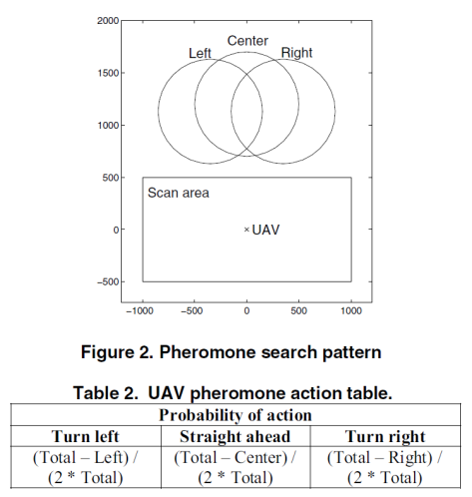
\includegraphics{../images/pheromon_model.png}
\end{center}

Nous avons traité tous les cas décrits dans l'article, c'est à dire que le noeud regarde les valeurs des phéromones en diagonale gauche, devant lui, en diagonale droite.\\\\

Une autre caractéristique de notre implémentation est que cette fois-ci, nous ne scannons plus un point de la carte mais les 5 décrits précédemment.\\\\

We handled all the cases described in the article, that is the node looks at the values of pheromones in its left diagonal, in front of him and in its right diagonal.

\begin{figure}[h]
\center
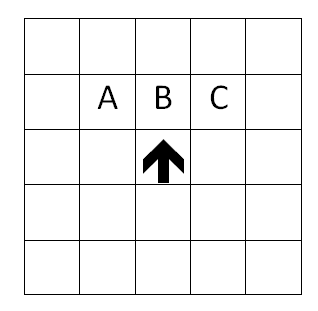
\includegraphics[width=5cm]{../images/grille_case_1.png}
\caption{case 1}
\end{figure}

\begin{figure}[h]
\center
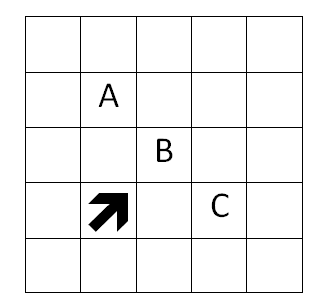
\includegraphics[width=5cm]{../images/grille_case_2.png}
\caption{case 2}
\end{figure}

These both case show how a node scan the map.
\begin{itemize}
\item the area A represents the left diagonal of the node.
\item the area B represents the front of the node.
\item the area C represents the right diagonal of the node.
\end{itemize}

Another characteristic of our implementation is that this time, we do not scan any more a point of the map but 5 described previously  like the picture below.

\begin{figure}[h]
\center
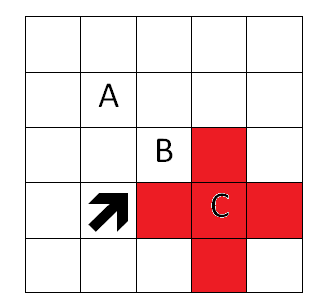
\includegraphics[width=5cm]{../images/grille_case_2_scan.png}
\caption{scan of area C}
\end{figure}

\textbf{A COMPLETER}



\section{Difficulties Encountered \& Solutions}

Au niveau de l'implémentation, nous n'avons pas rencontré beaucoup de difficultés. Le seul gros problème est l'affichage des zones scannées. Sur les conseils de Monsieur Casteigts, nous avons dû créer une classe héritant de JTopology et redéfinir la méthode \textit{paint}. En effet, le rafraichissement de l'affichage des zones scannées est un problème car nous perdions les zones scannées précédemment. Nous avons donc créé une ArrayList pour sauvegarder les zones scannées pour les redessiner à chaque fois.\\\\

La plus grosse difficultés rencontrées a été la lecture des nombreux articles en correspondance avec notre article d'étude. Ils comportaient de nombreuses pages et la lecture de ceux-ci en Anglais nous a prit énormément de temps. Nous avons dû par la suite mettre à jour les articles lus en recherchant sur internet les mises à jour.

Concerning the implementation, we did not meet many difficulties. The only big problem is the display of the scanned zones. On the advice of Mister Casteigts, we had to create a class inheriting from JTopology and redefine the method \textit{paint}. Indeed, the refreshment of the display of the scanned zones is a problem because we lost zones scanned previously. We created a ArrayList to save area scanned to redraw them in every times. \\\\
